% Options for packages loaded elsewhere
\PassOptionsToPackage{unicode}{hyperref}
\PassOptionsToPackage{hyphens}{url}
%
\documentclass[
]{article}
\usepackage{amsmath,amssymb}
\usepackage{lmodern}
\usepackage{iftex}
\ifPDFTeX
  \usepackage[T1]{fontenc}
  \usepackage[utf8]{inputenc}
  \usepackage{textcomp} % provide euro and other symbols
\else % if luatex or xetex
  \usepackage{unicode-math}
  \defaultfontfeatures{Scale=MatchLowercase}
  \defaultfontfeatures[\rmfamily]{Ligatures=TeX,Scale=1}
\fi
% Use upquote if available, for straight quotes in verbatim environments
\IfFileExists{upquote.sty}{\usepackage{upquote}}{}
\IfFileExists{microtype.sty}{% use microtype if available
  \usepackage[]{microtype}
  \UseMicrotypeSet[protrusion]{basicmath} % disable protrusion for tt fonts
}{}
\makeatletter
\@ifundefined{KOMAClassName}{% if non-KOMA class
  \IfFileExists{parskip.sty}{%
    \usepackage{parskip}
  }{% else
    \setlength{\parindent}{0pt}
    \setlength{\parskip}{6pt plus 2pt minus 1pt}}
}{% if KOMA class
  \KOMAoptions{parskip=half}}
\makeatother
\usepackage{xcolor}
\usepackage[margin=1in]{geometry}
\usepackage{color}
\usepackage{fancyvrb}
\newcommand{\VerbBar}{|}
\newcommand{\VERB}{\Verb[commandchars=\\\{\}]}
\DefineVerbatimEnvironment{Highlighting}{Verbatim}{commandchars=\\\{\}}
% Add ',fontsize=\small' for more characters per line
\usepackage{framed}
\definecolor{shadecolor}{RGB}{248,248,248}
\newenvironment{Shaded}{\begin{snugshade}}{\end{snugshade}}
\newcommand{\AlertTok}[1]{\textcolor[rgb]{0.94,0.16,0.16}{#1}}
\newcommand{\AnnotationTok}[1]{\textcolor[rgb]{0.56,0.35,0.01}{\textbf{\textit{#1}}}}
\newcommand{\AttributeTok}[1]{\textcolor[rgb]{0.77,0.63,0.00}{#1}}
\newcommand{\BaseNTok}[1]{\textcolor[rgb]{0.00,0.00,0.81}{#1}}
\newcommand{\BuiltInTok}[1]{#1}
\newcommand{\CharTok}[1]{\textcolor[rgb]{0.31,0.60,0.02}{#1}}
\newcommand{\CommentTok}[1]{\textcolor[rgb]{0.56,0.35,0.01}{\textit{#1}}}
\newcommand{\CommentVarTok}[1]{\textcolor[rgb]{0.56,0.35,0.01}{\textbf{\textit{#1}}}}
\newcommand{\ConstantTok}[1]{\textcolor[rgb]{0.00,0.00,0.00}{#1}}
\newcommand{\ControlFlowTok}[1]{\textcolor[rgb]{0.13,0.29,0.53}{\textbf{#1}}}
\newcommand{\DataTypeTok}[1]{\textcolor[rgb]{0.13,0.29,0.53}{#1}}
\newcommand{\DecValTok}[1]{\textcolor[rgb]{0.00,0.00,0.81}{#1}}
\newcommand{\DocumentationTok}[1]{\textcolor[rgb]{0.56,0.35,0.01}{\textbf{\textit{#1}}}}
\newcommand{\ErrorTok}[1]{\textcolor[rgb]{0.64,0.00,0.00}{\textbf{#1}}}
\newcommand{\ExtensionTok}[1]{#1}
\newcommand{\FloatTok}[1]{\textcolor[rgb]{0.00,0.00,0.81}{#1}}
\newcommand{\FunctionTok}[1]{\textcolor[rgb]{0.00,0.00,0.00}{#1}}
\newcommand{\ImportTok}[1]{#1}
\newcommand{\InformationTok}[1]{\textcolor[rgb]{0.56,0.35,0.01}{\textbf{\textit{#1}}}}
\newcommand{\KeywordTok}[1]{\textcolor[rgb]{0.13,0.29,0.53}{\textbf{#1}}}
\newcommand{\NormalTok}[1]{#1}
\newcommand{\OperatorTok}[1]{\textcolor[rgb]{0.81,0.36,0.00}{\textbf{#1}}}
\newcommand{\OtherTok}[1]{\textcolor[rgb]{0.56,0.35,0.01}{#1}}
\newcommand{\PreprocessorTok}[1]{\textcolor[rgb]{0.56,0.35,0.01}{\textit{#1}}}
\newcommand{\RegionMarkerTok}[1]{#1}
\newcommand{\SpecialCharTok}[1]{\textcolor[rgb]{0.00,0.00,0.00}{#1}}
\newcommand{\SpecialStringTok}[1]{\textcolor[rgb]{0.31,0.60,0.02}{#1}}
\newcommand{\StringTok}[1]{\textcolor[rgb]{0.31,0.60,0.02}{#1}}
\newcommand{\VariableTok}[1]{\textcolor[rgb]{0.00,0.00,0.00}{#1}}
\newcommand{\VerbatimStringTok}[1]{\textcolor[rgb]{0.31,0.60,0.02}{#1}}
\newcommand{\WarningTok}[1]{\textcolor[rgb]{0.56,0.35,0.01}{\textbf{\textit{#1}}}}
\usepackage{longtable,booktabs,array}
\usepackage{calc} % for calculating minipage widths
% Correct order of tables after \paragraph or \subparagraph
\usepackage{etoolbox}
\makeatletter
\patchcmd\longtable{\par}{\if@noskipsec\mbox{}\fi\par}{}{}
\makeatother
% Allow footnotes in longtable head/foot
\IfFileExists{footnotehyper.sty}{\usepackage{footnotehyper}}{\usepackage{footnote}}
\makesavenoteenv{longtable}
\usepackage{graphicx}
\makeatletter
\def\maxwidth{\ifdim\Gin@nat@width>\linewidth\linewidth\else\Gin@nat@width\fi}
\def\maxheight{\ifdim\Gin@nat@height>\textheight\textheight\else\Gin@nat@height\fi}
\makeatother
% Scale images if necessary, so that they will not overflow the page
% margins by default, and it is still possible to overwrite the defaults
% using explicit options in \includegraphics[width, height, ...]{}
\setkeys{Gin}{width=\maxwidth,height=\maxheight,keepaspectratio}
% Set default figure placement to htbp
\makeatletter
\def\fps@figure{htbp}
\makeatother
\setlength{\emergencystretch}{3em} % prevent overfull lines
\providecommand{\tightlist}{%
  \setlength{\itemsep}{0pt}\setlength{\parskip}{0pt}}
\setcounter{secnumdepth}{-\maxdimen} % remove section numbering
\ifLuaTeX
  \usepackage{selnolig}  % disable illegal ligatures
\fi
\IfFileExists{bookmark.sty}{\usepackage{bookmark}}{\usepackage{hyperref}}
\IfFileExists{xurl.sty}{\usepackage{xurl}}{} % add URL line breaks if available
\urlstyle{same} % disable monospaced font for URLs
\hypersetup{
  pdftitle={ExercisesAndAnswers},
  pdfauthor={You!},
  hidelinks,
  pdfcreator={LaTeX via pandoc}}

\title{ExercisesAndAnswers}
\author{You!}
\date{2023-02-27}

\begin{document}
\maketitle

\hypertarget{question-1}{%
\section{Question 1}\label{question-1}}

\includegraphics{}

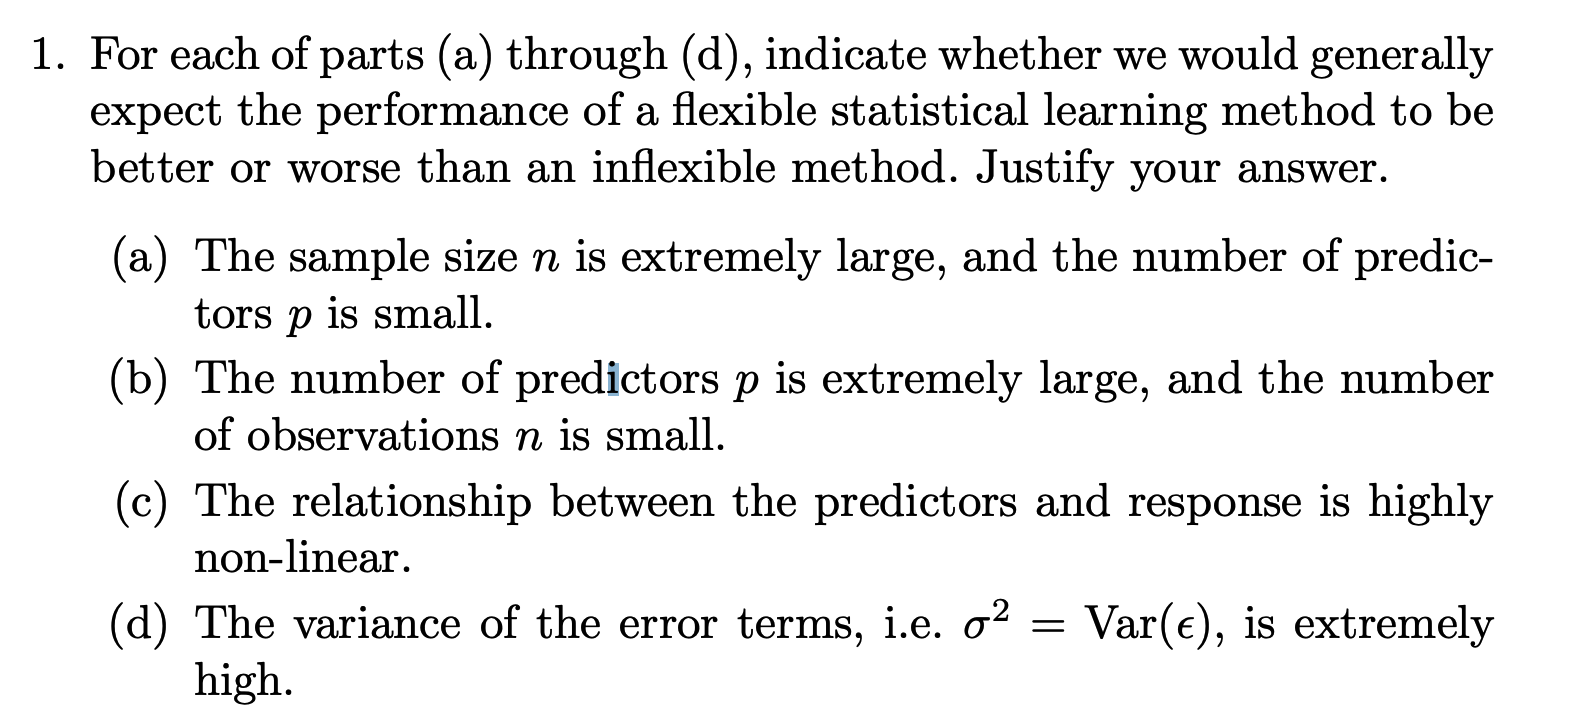
\includegraphics{images/image-1497375224.png}

\hypertarget{a}{%
\subsection{a)}\label{a}}

Flexible statistical Learning method is \textbf{BETTER}

A flexible statistical learning methods, such as random forest tree,
neural network, are able to capture complex relationship between
predictors and response.

\hypertarget{b}{%
\subsection{b)}\label{b}}

A flexible statistical learning method is \textbf{WORSE}

A flexible statistical learning methods, maybe suffer from
\textbf{OVERFITTING} problem, which can result in poor generalization
performance.

Inflexible methods can also provide interpretable models that can be
useful for understanding the \textbf{relationships} between predictors
and the response variable.

\hypertarget{c}{%
\subsection{c)}\label{c}}

A flexible statistical learning method is \textbf{BETTER}

A flexible statistical learning methods like tree-based models, neural
networks, and nonparametric regression methods have the ability to
capture non-linear relationships and interactions between variables,
which can be difficult or impossible for inflexible methods like linear
regression or logistic regression.

\hypertarget{d}{%
\subsection{d)}\label{d}}

A flexible statistical learning method is \textbf{WORSE}

A flexible statistical learning methods may fit the noise(outier) and
cause high variance.

\hypertarget{question-2}{%
\section{Question 2}\label{question-2}}

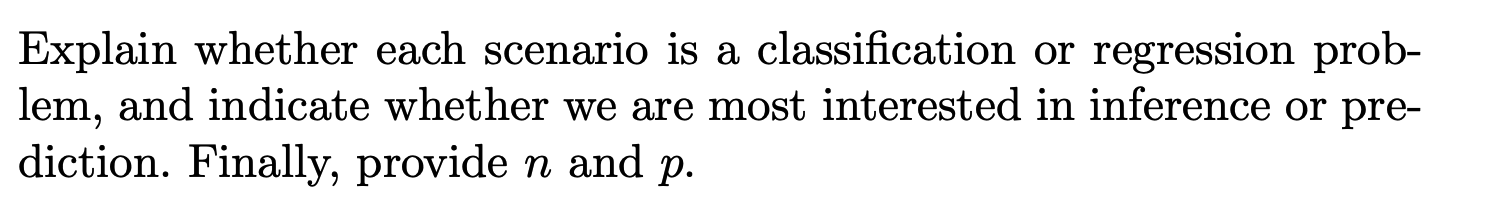
\includegraphics{images/image-2069609319.png}

\hypertarget{a-1}{%
\subsection{a)}\label{a-1}}

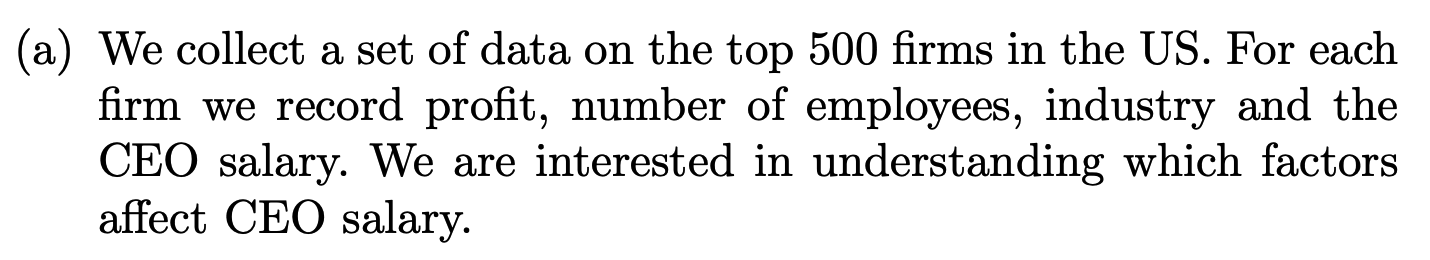
\includegraphics{images/image-1100398168.png}

Regression Problem

Inference Problem

n = 500

p = 3 (profit, number of employees, industry)

\hypertarget{b-1}{%
\subsection{b)}\label{b-1}}

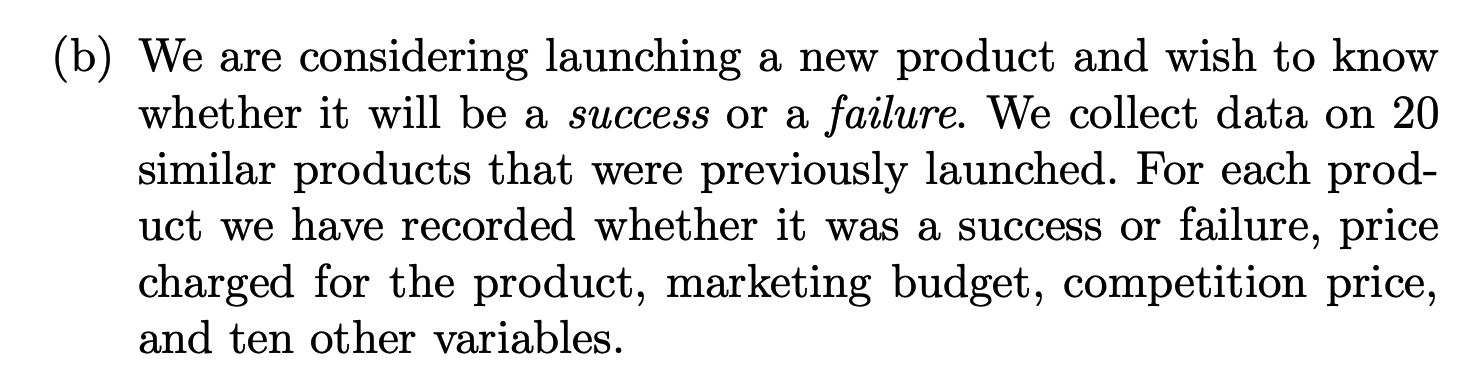
\includegraphics{images/image-1328812267.png}

Classification Problem

Prediction Problem

n = 20

p = 13(price charged for the product, marketing budget, competition
price, ten other variables)

\hypertarget{c-1}{%
\subsection{c)}\label{c-1}}

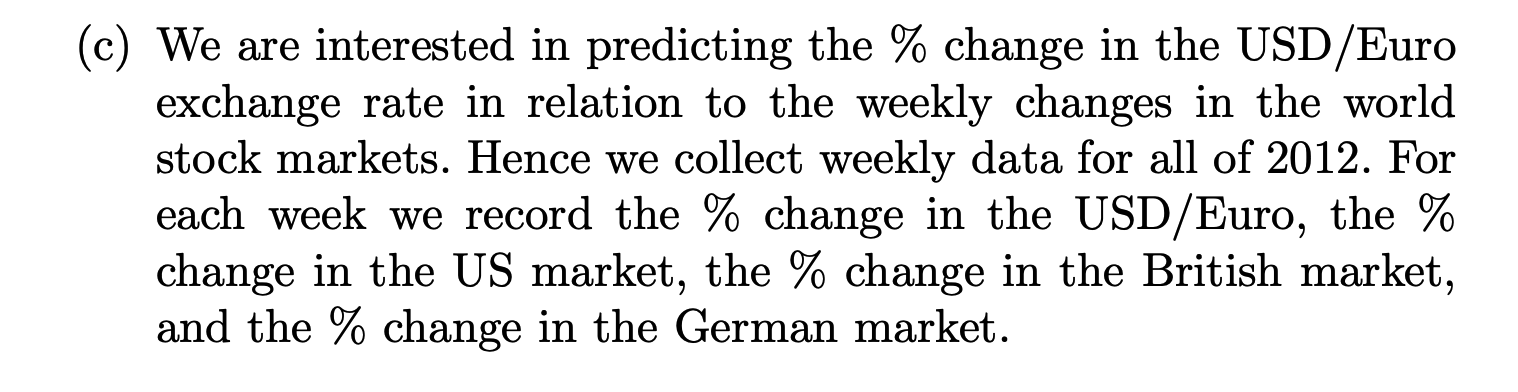
\includegraphics{images/image-827378815.png}

Regression Problem

Prediction Problem

n = 52 ( 52 weeks in 2012)

p = 3 (\% change in the US market, \% change in the British market, \%
change in the German market)

\hypertarget{question-3}{%
\section{Question 3}\label{question-3}}

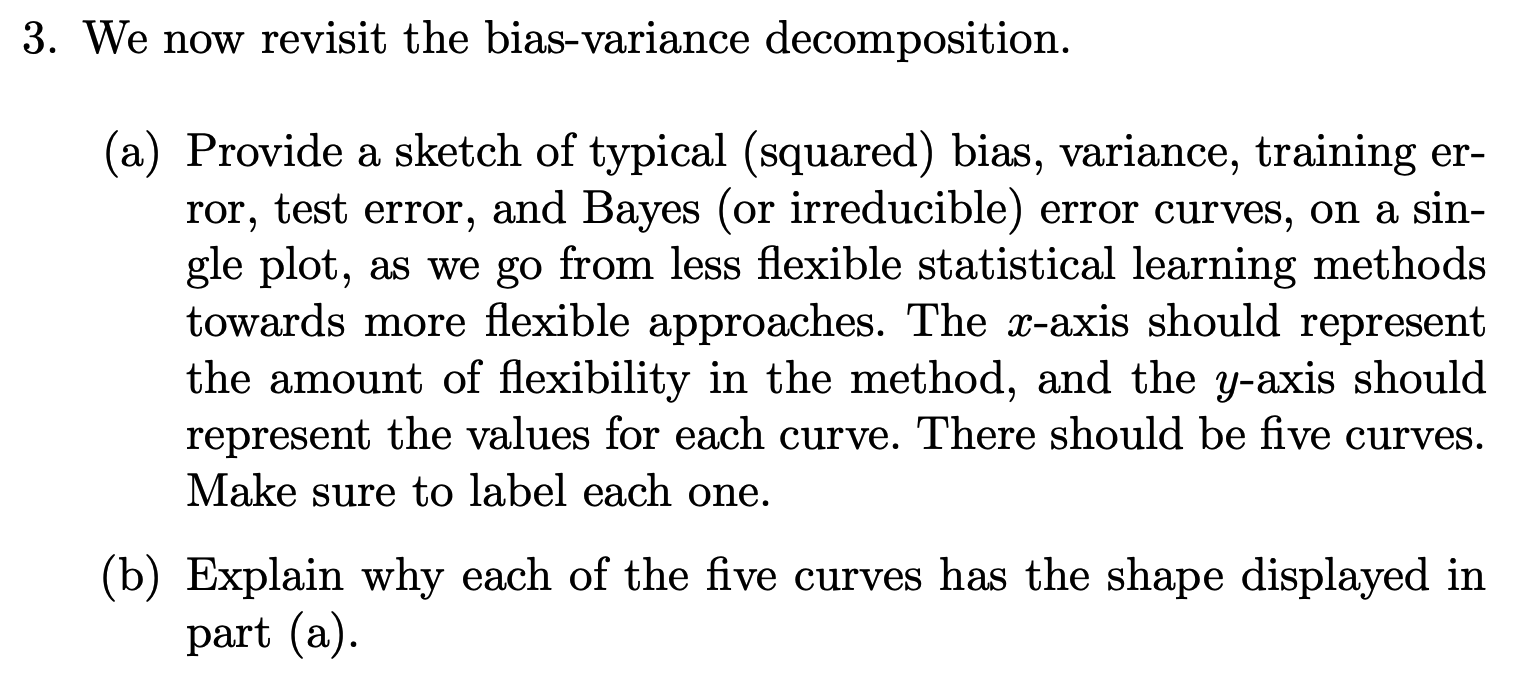
\includegraphics{images/image-997866889.png}

\hypertarget{a-2}{%
\subsection{a)}\label{a-2}}

\hypertarget{section}{%
\section{\texorpdfstring{\protect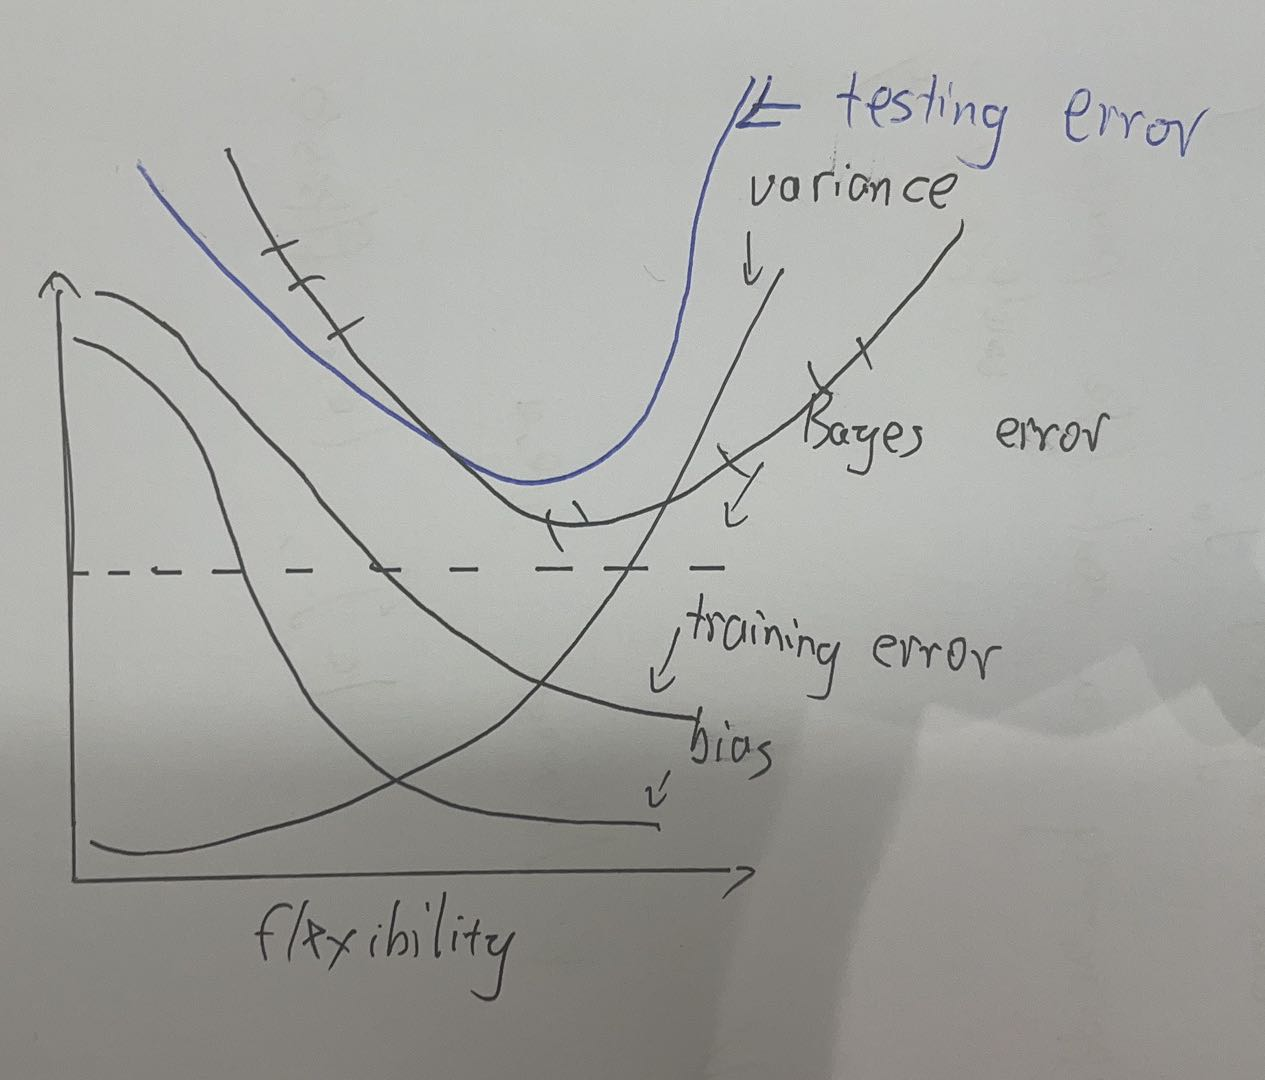
\includegraphics[width=8.41667in,height=4.32292in]{images/C2E3a.jpeg}}{}}\label{section}}

\hypertarget{b-2}{%
\subsection{b)}\label{b-2}}

Bias: Bias refers to the error that is introduced by approximating a
real-life problem with a simpler model. High bias means UNDERFITTING,
which means fail to capture the underlying patterns. As the flexibility
of model increases, the bias \textbf{decreases}.

Variance: Variance refers to the error that is introduced by the model;s
sensitivity on the fluctuations in the training data. High variance
means OVERFITTING, where the model fits the training data too closely
and fails to generalize to new data. As the flexibility of model
decrease, the variance \textbf{increase} as well

Training Error: With the flexibility of the model increases, the
training error tends to decrease as the model become more capable of
fitting the training data.

Test Error: With the flexibility of the model increases, the test error
initially decreases because the bias decrease more quickly, later the
variance increase more quickly then the bias decrease. So the test error
increase.

Bayes: It is the ir-reducible error, which is the lowest error that can
be achieved for a given problem. As the flexibility of the model
increase, the Bayes error will remain constant, as it is determined by
the inherent complexity of the problem, rather than the model's
flexibility.

\hypertarget{question-4}{%
\section{Question 4}\label{question-4}}

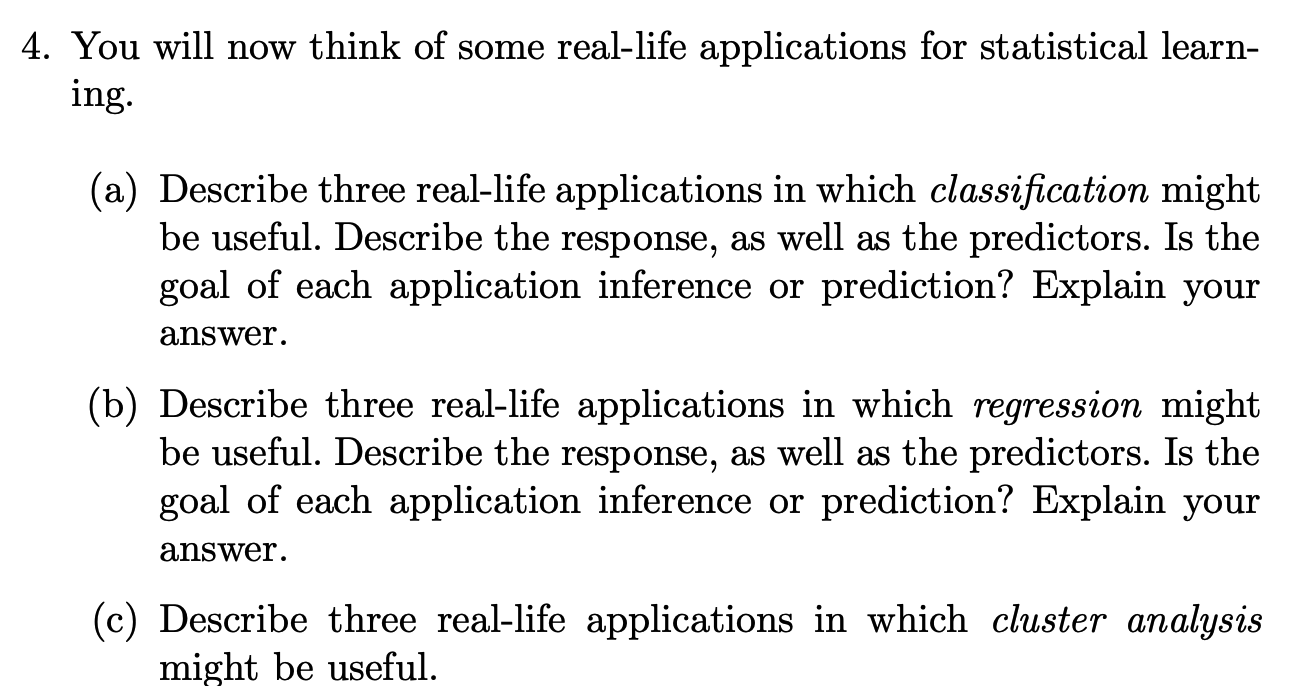
\includegraphics{images/image-1036292975.png}

\hypertarget{a-3}{%
\subsection{a)}\label{a-3}}

\begin{enumerate}
\def\labelenumi{\arabic{enumi}.}
\item
  Credit Scoring: Used by banks and other financial institution to
  assess the creditworthiness of load application.

  Response variable: Whether the load applications is likely to default
  to loan or not

  Predictors:

  \begin{itemize}
  \item
    income
  \item
    credit history
  \item
    employment status
  \item
    \ldots{}
  \end{itemize}

  It is the prediction problem
\item
  Medical Diagnosis: Used by healthcare providers to diagnose disease
  status based on patient symptoms and medical history

  Response Variable: The patient; disease status

  Predictors:

  \begin{itemize}
  \item
    age
  \item
    gender
  \item
    medical history
  \item
    \ldots{}
  \end{itemize}

  It is the prediction problem
\item
  Spam Email Filtering: Used by email service provider to filter out
  unwanted emails from the user's inbox

  Response Variable: Whether the email is Spam

  Predictors:

  \begin{itemize}
  \item
    email sender:
  \item
    subject line
  \item
    attachments
  \item
    \ldots{}
  \end{itemize}

  It is the prediction problem
\end{enumerate}

\hypertarget{b-3}{%
\subsection{b)}\label{b-3}}

\begin{enumerate}
\def\labelenumi{\arabic{enumi}.}
\item
  House Price Prediction:

  Response: Hose Price

  Predictors:

  \begin{itemize}
  \item
    House Size
  \item
    House Location
  \item
    House Age
  \item
    \ldots{}
  \end{itemize}

  Prediction Problem
\item
  Sales Forecasting:

  Response: sales volume

  Predictors:

  \begin{itemize}
  \item
    advertising expenditure
  \item
    pricing strategy
  \item
    seasonality
  \item
    \ldots.
  \end{itemize}

  Prediction Problem
\item
  Medical Cost Estimation:

  Response: cost of medical treatment

  Predictors:

  \begin{itemize}
  \item
    age
  \item
    gender
  \item
    medical history
  \item
    \ldots{}
  \end{itemize}

  Prediction Problem
\end{enumerate}

\hypertarget{c-2}{%
\subsection{c)}\label{c-2}}

\begin{enumerate}
\def\labelenumi{\arabic{enumi}.}
\tightlist
\item
  Customer Segmentation: Used by businesses to group customers based on
  their characteristics. To tailor marketing strategies and product
  offerings to each segment
\item
  Image Segmentation: Used in Computer Vision to group pixels in an
  image into homogeneous regions based on their color or texture. The
  goal is to identify regions in an image that have similar properties
  and can be treated as a seperateentity of further processing
\item
  Crime Hotspot Analysis: Used by law enforcement agencies to identify
  areas with a high frequency of crime incidents. The goal is to
  identify spatial clusters of crime incidents and allocate resources
  and law enforcement measures to reduce crime rates in these hotspots
\end{enumerate}

\hypertarget{question-5}{%
\section{Question 5}\label{question-5}}

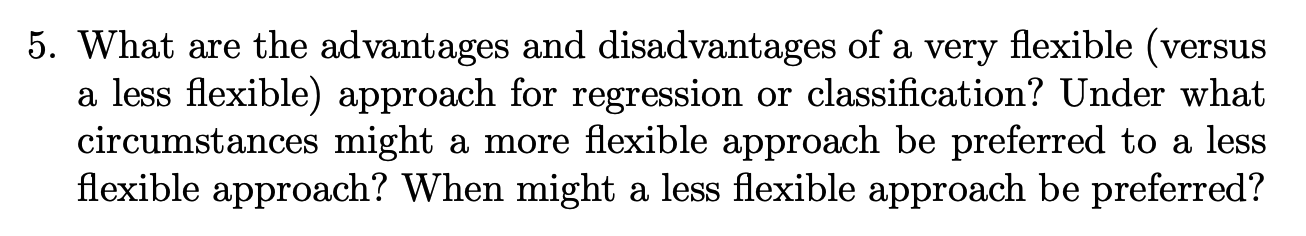
\includegraphics{images/image-44460808.png}

Advantages:

\begin{enumerate}
\def\labelenumi{\arabic{enumi}.}
\tightlist
\item
  capture complex and non-linear relationships between the predictors
  and the response
\item
  provide high accuracy on the training data
\end{enumerate}

Disadvantages:

\begin{enumerate}
\def\labelenumi{\arabic{enumi}.}
\tightlist
\item
  Prone to overfitting
\item
  Computationally expensive and require a large number of parameter
\end{enumerate}

A more flexible approach be preferred when:

\begin{enumerate}
\def\labelenumi{\arabic{enumi}.}
\tightlist
\item
  True relationship between the predictors and the response is complex
  and non-linear
\item
  The goal is to achieve high accuracy
\item
  Focus on Prediction rather than inference
\end{enumerate}

A less flexible approach be preferred when:

\begin{enumerate}
\def\labelenumi{\arabic{enumi}.}
\tightlist
\item
  true relationship between the predictors and the response is simple
  and linear
\item
  When the sample size is small
\item
  The Interpretation of the model is a primary concern, and is inference
  problem
\end{enumerate}

\hypertarget{question-6}{%
\section{Question 6}\label{question-6}}

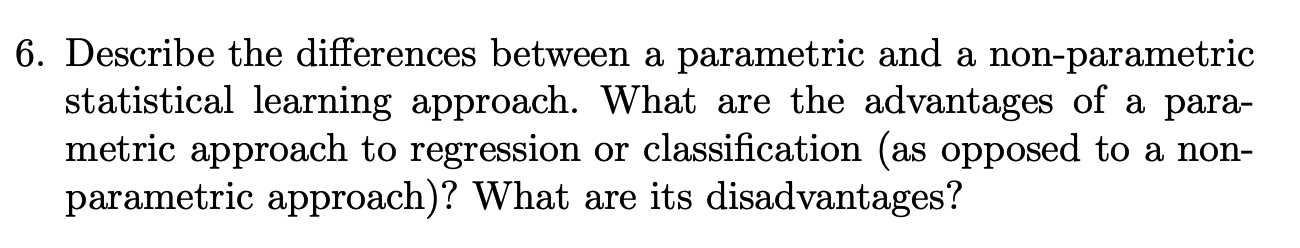
\includegraphics{images/image-1010253318.png}

A parametric statistical learning approach assumes a specific functional
form for the relationship between the predictors and the response, while
non-parameter statistical learning approach does not assume a specific
functional form for the relationship between predictors and the response
variable, and estimate the relationship directly from the data

Advantages of a parametric approach:

\begin{enumerate}
\def\labelenumi{\arabic{enumi}.}
\tightlist
\item
  More interpretable and easier to understand
\item
  Require less data to estimate their parameters
\item
  Provide more stable and precise estimates of the relationship between
  the predictors and the response
\end{enumerate}

Disadvantages of a parametric approach:

\begin{enumerate}
\def\labelenumi{\arabic{enumi}.}
\tightlist
\item
  May not capture complex or non-linear relationship between the
  predictors and the response.
\item
  Are sensitive to model misspecification, which occurs when true
  relationship between the predictors and the response deviates from the
  assumed functional form
\item
  May be biased if the assumptions of the model are violated or the data
  is not representative the population
\end{enumerate}

\hypertarget{question-7}{%
\section{Question 7}\label{question-7}}

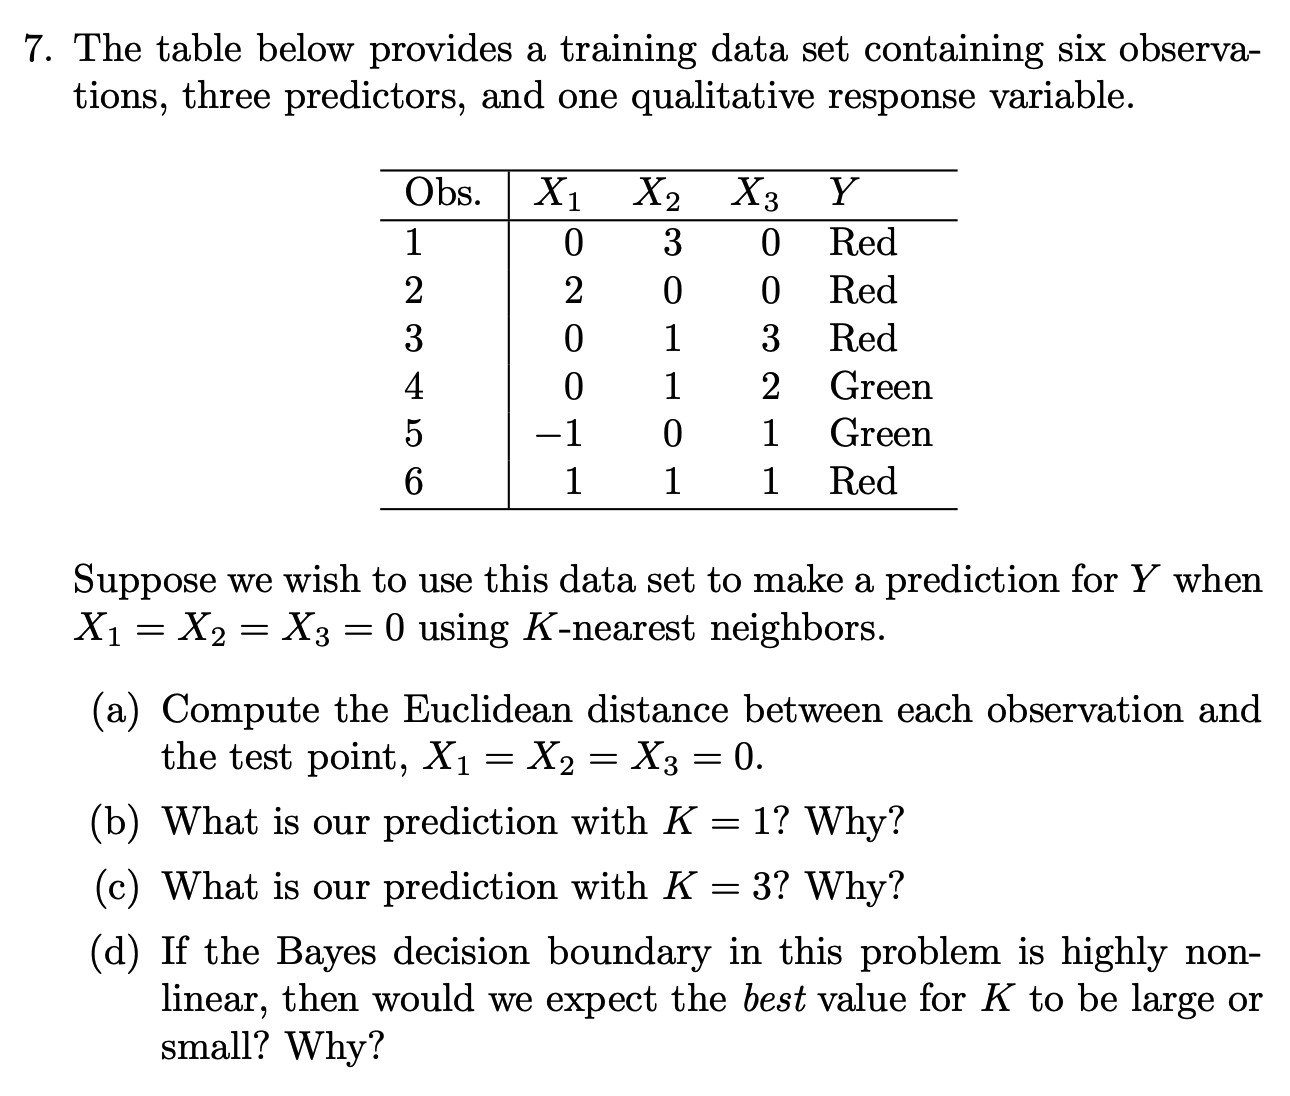
\includegraphics{images/image-1787682983.png}

\hypertarget{a-4}{%
\subsection{a)}\label{a-4}}

Euclidean Distance:

Distance = sqrt( (x2-x1) \^{} 2 + (y2-y1) \^{} 2 )

\begin{longtable}[]{@{}lll@{}}
\toprule()
Obs & Distance \^{} 2 & Y \\
\midrule()
\endhead
1 & 9 & Red \\
2 & 4 & Red \\
3 & 10 & Red \\
4 & 5 & Green \\
5 & 2 & Green \\
6 & 3 & Red \\
\bottomrule()
\end{longtable}

\hypertarget{b-4}{%
\subsection{b)}\label{b-4}}

Green

\hypertarget{c-3}{%
\subsection{c)}\label{c-3}}

Red

\hypertarget{d-1}{%
\subsection{d)}\label{d-1}}

Small. A small K would be flexible for a non-linear decision boundary.

\hypertarget{question-8}{%
\section{Question 8}\label{question-8}}

\hypertarget{a-5}{%
\subsection{a)}\label{a-5}}

\begin{Shaded}
\begin{Highlighting}[]
\NormalTok{college }\OtherTok{\textless{}{-}} \FunctionTok{read.csv}\NormalTok{(}\StringTok{"College.csv"}\NormalTok{)}
\end{Highlighting}
\end{Shaded}

\hypertarget{b-5}{%
\subsection{b)}\label{b-5}}

\begin{Shaded}
\begin{Highlighting}[]
\FunctionTok{head}\NormalTok{(college)}
\end{Highlighting}
\end{Shaded}

\begin{verbatim}
##                              X Private Apps Accept Enroll Top10perc Top25perc
## 1 Abilene Christian University     Yes 1660   1232    721        23        52
## 2           Adelphi University     Yes 2186   1924    512        16        29
## 3               Adrian College     Yes 1428   1097    336        22        50
## 4          Agnes Scott College     Yes  417    349    137        60        89
## 5    Alaska Pacific University     Yes  193    146     55        16        44
## 6            Albertson College     Yes  587    479    158        38        62
##   F.Undergrad P.Undergrad Outstate Room.Board Books Personal PhD Terminal
## 1        2885         537     7440       3300   450     2200  70       78
## 2        2683        1227    12280       6450   750     1500  29       30
## 3        1036          99    11250       3750   400     1165  53       66
## 4         510          63    12960       5450   450      875  92       97
## 5         249         869     7560       4120   800     1500  76       72
## 6         678          41    13500       3335   500      675  67       73
##   S.F.Ratio perc.alumni Expend Grad.Rate
## 1      18.1          12   7041        60
## 2      12.2          16  10527        56
## 3      12.9          30   8735        54
## 4       7.7          37  19016        59
## 5      11.9           2  10922        15
## 6       9.4          11   9727        55
\end{verbatim}

\begin{Shaded}
\begin{Highlighting}[]
\CommentTok{\# First Column just the name of each university, need remove this columns}
\CommentTok{\# Store the Row Name first}
\FunctionTok{rownames}\NormalTok{(college) }\OtherTok{\textless{}{-}}\NormalTok{ college[,}\DecValTok{1}\NormalTok{]}
\CommentTok{\# View(college)}
\CommentTok{\# Elimate the first column}
\NormalTok{college }\OtherTok{\textless{}{-}}\NormalTok{ college[, }\SpecialCharTok{{-}}\DecValTok{1}\NormalTok{]}
\FunctionTok{View}\NormalTok{(college)}
\end{Highlighting}
\end{Shaded}

\hypertarget{c-4}{%
\subsection{c)}\label{c-4}}

\begin{Shaded}
\begin{Highlighting}[]
\FunctionTok{summary}\NormalTok{(college)}
\end{Highlighting}
\end{Shaded}

\begin{verbatim}
##    Private               Apps           Accept          Enroll    
##  Length:777         Min.   :   81   Min.   :   72   Min.   :  35  
##  Class :character   1st Qu.:  776   1st Qu.:  604   1st Qu.: 242  
##  Mode  :character   Median : 1558   Median : 1110   Median : 434  
##                     Mean   : 3002   Mean   : 2019   Mean   : 780  
##                     3rd Qu.: 3624   3rd Qu.: 2424   3rd Qu.: 902  
##                     Max.   :48094   Max.   :26330   Max.   :6392  
##    Top10perc       Top25perc      F.Undergrad     P.Undergrad     
##  Min.   : 1.00   Min.   :  9.0   Min.   :  139   Min.   :    1.0  
##  1st Qu.:15.00   1st Qu.: 41.0   1st Qu.:  992   1st Qu.:   95.0  
##  Median :23.00   Median : 54.0   Median : 1707   Median :  353.0  
##  Mean   :27.56   Mean   : 55.8   Mean   : 3700   Mean   :  855.3  
##  3rd Qu.:35.00   3rd Qu.: 69.0   3rd Qu.: 4005   3rd Qu.:  967.0  
##  Max.   :96.00   Max.   :100.0   Max.   :31643   Max.   :21836.0  
##     Outstate       Room.Board       Books           Personal   
##  Min.   : 2340   Min.   :1780   Min.   :  96.0   Min.   : 250  
##  1st Qu.: 7320   1st Qu.:3597   1st Qu.: 470.0   1st Qu.: 850  
##  Median : 9990   Median :4200   Median : 500.0   Median :1200  
##  Mean   :10441   Mean   :4358   Mean   : 549.4   Mean   :1341  
##  3rd Qu.:12925   3rd Qu.:5050   3rd Qu.: 600.0   3rd Qu.:1700  
##  Max.   :21700   Max.   :8124   Max.   :2340.0   Max.   :6800  
##       PhD            Terminal       S.F.Ratio      perc.alumni   
##  Min.   :  8.00   Min.   : 24.0   Min.   : 2.50   Min.   : 0.00  
##  1st Qu.: 62.00   1st Qu.: 71.0   1st Qu.:11.50   1st Qu.:13.00  
##  Median : 75.00   Median : 82.0   Median :13.60   Median :21.00  
##  Mean   : 72.66   Mean   : 79.7   Mean   :14.09   Mean   :22.74  
##  3rd Qu.: 85.00   3rd Qu.: 92.0   3rd Qu.:16.50   3rd Qu.:31.00  
##  Max.   :103.00   Max.   :100.0   Max.   :39.80   Max.   :64.00  
##      Expend        Grad.Rate     
##  Min.   : 3186   Min.   : 10.00  
##  1st Qu.: 6751   1st Qu.: 53.00  
##  Median : 8377   Median : 65.00  
##  Mean   : 9660   Mean   : 65.46  
##  3rd Qu.:10830   3rd Qu.: 78.00  
##  Max.   :56233   Max.   :118.00
\end{verbatim}

\begin{Shaded}
\begin{Highlighting}[]
\NormalTok{college[,}\DecValTok{1}\NormalTok{] }\OtherTok{=} \FunctionTok{as.numeric}\NormalTok{(}\FunctionTok{factor}\NormalTok{(college[,}\DecValTok{1}\NormalTok{]))}
\FunctionTok{pairs}\NormalTok{(college[,}\DecValTok{1}\SpecialCharTok{:}\DecValTok{10}\NormalTok{])}
\end{Highlighting}
\end{Shaded}

\includegraphics{ExerciseAndAnswers_files/figure-latex/unnamed-chunk-3-1.pdf}

\begin{Shaded}
\begin{Highlighting}[]
\CommentTok{\# iii}
\FunctionTok{plot}\NormalTok{(college}\SpecialCharTok{$}\NormalTok{Outstate, college}\SpecialCharTok{$}\NormalTok{Outstate)}
\end{Highlighting}
\end{Shaded}

\includegraphics{ExerciseAndAnswers_files/figure-latex/unnamed-chunk-4-1.pdf}

\begin{Shaded}
\begin{Highlighting}[]
\NormalTok{Elite }\OtherTok{\textless{}{-}} \FunctionTok{rep}\NormalTok{(}\StringTok{"No"}\NormalTok{, }\FunctionTok{nrow}\NormalTok{(college))}
\NormalTok{Elite[college}\SpecialCharTok{$}\NormalTok{Top10perc }\SpecialCharTok{\textgreater{}} \DecValTok{50}\NormalTok{] }\OtherTok{\textless{}{-}} \StringTok{"Yes"}
\NormalTok{Elite }\OtherTok{\textless{}{-}} \FunctionTok{as.factor}\NormalTok{(Elite)}
\NormalTok{college }\OtherTok{\textless{}{-}} \FunctionTok{data.frame}\NormalTok{(college, Elite)}
\FunctionTok{summary}\NormalTok{(college}\SpecialCharTok{$}\NormalTok{Elite)}
\end{Highlighting}
\end{Shaded}

\begin{verbatim}
##  No Yes 
## 699  78
\end{verbatim}

\begin{Shaded}
\begin{Highlighting}[]
\FunctionTok{plot}\NormalTok{(college}\SpecialCharTok{$}\NormalTok{Outstate, college}\SpecialCharTok{$}\NormalTok{Elite)}
\end{Highlighting}
\end{Shaded}

\includegraphics{ExerciseAndAnswers_files/figure-latex/unnamed-chunk-5-1.pdf}

\begin{Shaded}
\begin{Highlighting}[]
\FunctionTok{par}\NormalTok{(}\AttributeTok{mfrow=}\FunctionTok{c}\NormalTok{(}\DecValTok{2}\NormalTok{,}\DecValTok{2}\NormalTok{))}
\FunctionTok{hist}\NormalTok{(college}\SpecialCharTok{$}\NormalTok{Apps)}
\FunctionTok{hist}\NormalTok{(college}\SpecialCharTok{$}\NormalTok{perc.alumni, }\AttributeTok{col=}\DecValTok{2}\NormalTok{)}
\FunctionTok{hist}\NormalTok{(college}\SpecialCharTok{$}\NormalTok{S.F.Ratio, }\AttributeTok{col=}\DecValTok{3}\NormalTok{, }\AttributeTok{breaks=}\DecValTok{10}\NormalTok{)}
\FunctionTok{hist}\NormalTok{(college}\SpecialCharTok{$}\NormalTok{Expend, }\AttributeTok{breaks=}\DecValTok{100}\NormalTok{)}
\end{Highlighting}
\end{Shaded}

\includegraphics{ExerciseAndAnswers_files/figure-latex/unnamed-chunk-6-1.pdf}

\begin{Shaded}
\begin{Highlighting}[]
\FunctionTok{par}\NormalTok{(}\AttributeTok{mfrow=}\FunctionTok{c}\NormalTok{(}\DecValTok{2}\NormalTok{,}\DecValTok{2}\NormalTok{))}
\FunctionTok{plot}\NormalTok{(college}\SpecialCharTok{$}\NormalTok{Outstate, college}\SpecialCharTok{$}\NormalTok{Grad.Rate)}
\CommentTok{\# High tuition correlates to high graduation rate.}
\FunctionTok{plot}\NormalTok{(college}\SpecialCharTok{$}\NormalTok{Accept }\SpecialCharTok{/}\NormalTok{ college}\SpecialCharTok{$}\NormalTok{Apps, college}\SpecialCharTok{$}\NormalTok{S.F.Ratio)}
\CommentTok{\# Colleges with low acceptance rate tend to have low S:F ratio.}
\FunctionTok{plot}\NormalTok{(college}\SpecialCharTok{$}\NormalTok{Top10perc, college}\SpecialCharTok{$}\NormalTok{Grad.Rate)}
\CommentTok{\# Colleges with the most students from top 10\% perc don\textquotesingle{}t necessarily have}
\CommentTok{\# the highest graduation rate. Also, rate \textgreater{} 100 is erroneous!}
\end{Highlighting}
\end{Shaded}

\includegraphics{ExerciseAndAnswers_files/figure-latex/unnamed-chunk-7-1.pdf}

\hypertarget{question-9}{%
\section{Question 9}\label{question-9}}

\hypertarget{a-6}{%
\subsection{a)}\label{a-6}}

\begin{Shaded}
\begin{Highlighting}[]
\CommentTok{\# Load Data }
\NormalTok{Auto }\OtherTok{\textless{}{-}} \FunctionTok{read.csv}\NormalTok{(}\StringTok{"Auto.csv"}\NormalTok{, }\AttributeTok{header =}\NormalTok{ T, }\AttributeTok{na.strings =} \StringTok{"?"}\NormalTok{)}
\CommentTok{\# Check if their is Na and remove the NA value}
\ControlFlowTok{if}\NormalTok{ (}\FunctionTok{any}\NormalTok{(}\FunctionTok{is.na}\NormalTok{(Auto)))\{}
\NormalTok{  Auto }\OtherTok{\textless{}{-}} \FunctionTok{na.omit}\NormalTok{(Auto)}
\NormalTok{\}}
\FunctionTok{dim}\NormalTok{(Auto)}
\end{Highlighting}
\end{Shaded}

\begin{verbatim}
## [1] 392   9
\end{verbatim}

\begin{Shaded}
\begin{Highlighting}[]
\FunctionTok{summary}\NormalTok{(Auto)}
\end{Highlighting}
\end{Shaded}

\begin{verbatim}
##       mpg          cylinders      displacement     horsepower        weight    
##  Min.   : 9.00   Min.   :3.000   Min.   : 68.0   Min.   : 46.0   Min.   :1613  
##  1st Qu.:17.00   1st Qu.:4.000   1st Qu.:105.0   1st Qu.: 75.0   1st Qu.:2225  
##  Median :22.75   Median :4.000   Median :151.0   Median : 93.5   Median :2804  
##  Mean   :23.45   Mean   :5.472   Mean   :194.4   Mean   :104.5   Mean   :2978  
##  3rd Qu.:29.00   3rd Qu.:8.000   3rd Qu.:275.8   3rd Qu.:126.0   3rd Qu.:3615  
##  Max.   :46.60   Max.   :8.000   Max.   :455.0   Max.   :230.0   Max.   :5140  
##   acceleration        year           origin          name          
##  Min.   : 8.00   Min.   :70.00   Min.   :1.000   Length:392        
##  1st Qu.:13.78   1st Qu.:73.00   1st Qu.:1.000   Class :character  
##  Median :15.50   Median :76.00   Median :1.000   Mode  :character  
##  Mean   :15.54   Mean   :75.98   Mean   :1.577                     
##  3rd Qu.:17.02   3rd Qu.:79.00   3rd Qu.:2.000                     
##  Max.   :24.80   Max.   :82.00   Max.   :3.000
\end{verbatim}

\textbf{Quantitative}: mpg, cylinders, displacement, horsepower, weight,
acceleration, year

\textbf{Qualitative}: name, origin

\hypertarget{b-6}{%
\subsection{b)}\label{b-6}}

\begin{Shaded}
\begin{Highlighting}[]
\FunctionTok{sapply}\NormalTok{(Auto[,}\DecValTok{1}\SpecialCharTok{:}\DecValTok{7}\NormalTok{], range)}
\end{Highlighting}
\end{Shaded}

\begin{verbatim}
##       mpg cylinders displacement horsepower weight acceleration year
## [1,]  9.0         3           68         46   1613          8.0   70
## [2,] 46.6         8          455        230   5140         24.8   82
\end{verbatim}

\hypertarget{c-5}{%
\subsection{c)}\label{c-5}}

\begin{Shaded}
\begin{Highlighting}[]
\FunctionTok{print}\NormalTok{(}\FunctionTok{sapply}\NormalTok{(Auto[,}\DecValTok{1}\SpecialCharTok{:}\DecValTok{7}\NormalTok{], mean))}
\end{Highlighting}
\end{Shaded}

\begin{verbatim}
##          mpg    cylinders displacement   horsepower       weight acceleration 
##    23.445918     5.471939   194.411990   104.469388  2977.584184    15.541327 
##         year 
##    75.979592
\end{verbatim}

\begin{Shaded}
\begin{Highlighting}[]
\FunctionTok{print}\NormalTok{(}\FunctionTok{sapply}\NormalTok{(Auto[,}\DecValTok{1}\SpecialCharTok{:}\DecValTok{7}\NormalTok{], sd))}
\end{Highlighting}
\end{Shaded}

\begin{verbatim}
##          mpg    cylinders displacement   horsepower       weight acceleration 
##     7.805007     1.705783   104.644004    38.491160   849.402560     2.758864 
##         year 
##     3.683737
\end{verbatim}

\hypertarget{d-2}{%
\subsection{d)}\label{d-2}}

\begin{Shaded}
\begin{Highlighting}[]
\CommentTok{\# Remove the 10th and 85th}
\NormalTok{newAuto }\OtherTok{\textless{}{-}}\NormalTok{ Auto[}\SpecialCharTok{{-}}\NormalTok{(}\DecValTok{10}\SpecialCharTok{:}\DecValTok{85}\NormalTok{),]}
\CommentTok{\# Check If remove success}
\FunctionTok{dim}\NormalTok{(newAuto) }\SpecialCharTok{==}\NormalTok{ (}\FunctionTok{dim}\NormalTok{(Auto) }\SpecialCharTok{{-}} \FunctionTok{c}\NormalTok{(}\DecValTok{76}\NormalTok{,}\DecValTok{0}\NormalTok{))}
\end{Highlighting}
\end{Shaded}

\begin{verbatim}
## [1] TRUE TRUE
\end{verbatim}

\begin{Shaded}
\begin{Highlighting}[]
\FunctionTok{sapply}\NormalTok{(newAuto[, }\DecValTok{1}\SpecialCharTok{:}\DecValTok{7}\NormalTok{], range)}
\end{Highlighting}
\end{Shaded}

\begin{verbatim}
##       mpg cylinders displacement horsepower weight acceleration year
## [1,] 11.0         3           68         46   1649          8.5   70
## [2,] 46.6         8          455        230   4997         24.8   82
\end{verbatim}

\begin{Shaded}
\begin{Highlighting}[]
\FunctionTok{sapply}\NormalTok{(newAuto[, }\DecValTok{1}\SpecialCharTok{:}\DecValTok{7}\NormalTok{], mean)}
\end{Highlighting}
\end{Shaded}

\begin{verbatim}
##          mpg    cylinders displacement   horsepower       weight acceleration 
##    24.404430     5.373418   187.240506   100.721519  2935.971519    15.726899 
##         year 
##    77.145570
\end{verbatim}

\begin{Shaded}
\begin{Highlighting}[]
\FunctionTok{sapply}\NormalTok{(newAuto[, }\DecValTok{1}\SpecialCharTok{:}\DecValTok{7}\NormalTok{], sd)}
\end{Highlighting}
\end{Shaded}

\begin{verbatim}
##          mpg    cylinders displacement   horsepower       weight acceleration 
##     7.867283     1.654179    99.678367    35.708853   811.300208     2.693721 
##         year 
##     3.106217
\end{verbatim}

\hypertarget{e}{%
\subsection{e)}\label{e}}

\begin{Shaded}
\begin{Highlighting}[]
\FunctionTok{library}\NormalTok{(corrgram)}
\FunctionTok{library}\NormalTok{(corrplot)}
\end{Highlighting}
\end{Shaded}

\begin{verbatim}
## corrplot 0.92 loaded
\end{verbatim}

\begin{Shaded}
\begin{Highlighting}[]
\FunctionTok{corrgram}\NormalTok{(Auto, }\AttributeTok{order=}\ConstantTok{TRUE}\NormalTok{, }
         \AttributeTok{panel =}\NormalTok{ panel.pie, }
         \AttributeTok{text.panel =}\NormalTok{ panel.txt}
\NormalTok{         )}
\end{Highlighting}
\end{Shaded}

\includegraphics{ExerciseAndAnswers_files/figure-latex/unnamed-chunk-15-1.pdf}

\hypertarget{f}{%
\subsection{f)}\label{f}}

all predictors have some correlation with mpg

\hypertarget{question-10}{%
\section{Question 10}\label{question-10}}

\hypertarget{a-7}{%
\subsection{a)}\label{a-7}}

\begin{Shaded}
\begin{Highlighting}[]
\FunctionTok{library}\NormalTok{(MASS) }\CommentTok{\# Data Set Also in MASS}
\FunctionTok{head}\NormalTok{(Boston) }
\end{Highlighting}
\end{Shaded}

\begin{verbatim}
##      crim zn indus chas   nox    rm  age    dis rad tax ptratio  black lstat
## 1 0.00632 18  2.31    0 0.538 6.575 65.2 4.0900   1 296    15.3 396.90  4.98
## 2 0.02731  0  7.07    0 0.469 6.421 78.9 4.9671   2 242    17.8 396.90  9.14
## 3 0.02729  0  7.07    0 0.469 7.185 61.1 4.9671   2 242    17.8 392.83  4.03
## 4 0.03237  0  2.18    0 0.458 6.998 45.8 6.0622   3 222    18.7 394.63  2.94
## 5 0.06905  0  2.18    0 0.458 7.147 54.2 6.0622   3 222    18.7 396.90  5.33
## 6 0.02985  0  2.18    0 0.458 6.430 58.7 6.0622   3 222    18.7 394.12  5.21
##   medv
## 1 24.0
## 2 21.6
## 3 34.7
## 4 33.4
## 5 36.2
## 6 28.7
\end{verbatim}

\begin{Shaded}
\begin{Highlighting}[]
\FunctionTok{dim}\NormalTok{(Boston) }\CommentTok{\# 506, 14}
\end{Highlighting}
\end{Shaded}

\begin{verbatim}
## [1] 506  14
\end{verbatim}

\hypertarget{b-7}{%
\subsection{b)}\label{b-7}}

\begin{Shaded}
\begin{Highlighting}[]
\FunctionTok{pairs}\NormalTok{(Boston)}
\end{Highlighting}
\end{Shaded}

\includegraphics{ExerciseAndAnswers_files/figure-latex/unnamed-chunk-17-1.pdf}

\hypertarget{c-6}{%
\subsection{c)}\label{c-6}}

\begin{Shaded}
\begin{Highlighting}[]
\FunctionTok{plot}\NormalTok{(Boston}\SpecialCharTok{$}\NormalTok{age, Boston}\SpecialCharTok{$}\NormalTok{crim)}
\end{Highlighting}
\end{Shaded}

\includegraphics{ExerciseAndAnswers_files/figure-latex/unnamed-chunk-18-1.pdf}

\begin{Shaded}
\begin{Highlighting}[]
\CommentTok{\# Older homes, more crime}
\FunctionTok{plot}\NormalTok{(Boston}\SpecialCharTok{$}\NormalTok{dis, Boston}\SpecialCharTok{$}\NormalTok{crim)}
\end{Highlighting}
\end{Shaded}

\includegraphics{ExerciseAndAnswers_files/figure-latex/unnamed-chunk-18-2.pdf}

\begin{Shaded}
\begin{Highlighting}[]
\CommentTok{\# Closer to work{-}area, more crime}
\FunctionTok{plot}\NormalTok{(Boston}\SpecialCharTok{$}\NormalTok{rad, Boston}\SpecialCharTok{$}\NormalTok{crim)}
\end{Highlighting}
\end{Shaded}

\includegraphics{ExerciseAndAnswers_files/figure-latex/unnamed-chunk-18-3.pdf}

\begin{Shaded}
\begin{Highlighting}[]
\CommentTok{\# Higher index of accessibility to radial highways, more crime}
\FunctionTok{plot}\NormalTok{(Boston}\SpecialCharTok{$}\NormalTok{tax, Boston}\SpecialCharTok{$}\NormalTok{crim)}
\end{Highlighting}
\end{Shaded}

\includegraphics{ExerciseAndAnswers_files/figure-latex/unnamed-chunk-18-4.pdf}

\begin{Shaded}
\begin{Highlighting}[]
\CommentTok{\# Higher tax rate, more crime}
\FunctionTok{plot}\NormalTok{(Boston}\SpecialCharTok{$}\NormalTok{ptratio, Boston}\SpecialCharTok{$}\NormalTok{crim)}
\end{Highlighting}
\end{Shaded}

\includegraphics{ExerciseAndAnswers_files/figure-latex/unnamed-chunk-18-5.pdf}

\begin{Shaded}
\begin{Highlighting}[]
\CommentTok{\# Higher pupil:teacher ratio, more crime}
\end{Highlighting}
\end{Shaded}

\hypertarget{d-3}{%
\subsection{d)}\label{d-3}}

\begin{Shaded}
\begin{Highlighting}[]
\FunctionTok{par}\NormalTok{(}\AttributeTok{mfrow=}\FunctionTok{c}\NormalTok{(}\DecValTok{1}\NormalTok{,}\DecValTok{3}\NormalTok{))}
\FunctionTok{hist}\NormalTok{(Boston}\SpecialCharTok{$}\NormalTok{crim[Boston}\SpecialCharTok{$}\NormalTok{crim}\SpecialCharTok{\textgreater{}}\DecValTok{1}\NormalTok{], }\AttributeTok{breaks=}\DecValTok{25}\NormalTok{)}
\CommentTok{\# most cities have low crime rates, but there is a long tail: 18 suburbs appear}
\CommentTok{\# to have a crime rate \textgreater{} 20, reaching to above 80}
\FunctionTok{hist}\NormalTok{(Boston}\SpecialCharTok{$}\NormalTok{tax, }\AttributeTok{breaks=}\DecValTok{25}\NormalTok{)}
\CommentTok{\# there is a large divide between suburbs with low tax rates and a peak at 660{-}680}
\FunctionTok{hist}\NormalTok{(Boston}\SpecialCharTok{$}\NormalTok{ptratio, }\AttributeTok{breaks=}\DecValTok{25}\NormalTok{)}
\end{Highlighting}
\end{Shaded}

\includegraphics{ExerciseAndAnswers_files/figure-latex/unnamed-chunk-19-1.pdf}

\begin{Shaded}
\begin{Highlighting}[]
\CommentTok{\# a skew towards high ratios, but no particularly high ratios}
\end{Highlighting}
\end{Shaded}

\hypertarget{e-1}{%
\subsection{e)}\label{e-1}}

\begin{Shaded}
\begin{Highlighting}[]
\FunctionTok{dim}\NormalTok{(}\FunctionTok{subset}\NormalTok{(Boston, chas }\SpecialCharTok{==} \DecValTok{1}\NormalTok{)) }\CommentTok{\# 35}
\end{Highlighting}
\end{Shaded}

\begin{verbatim}
## [1] 35 14
\end{verbatim}

\hypertarget{f-1}{%
\subsection{f)}\label{f-1}}

\begin{Shaded}
\begin{Highlighting}[]
\FunctionTok{median}\NormalTok{(Boston}\SpecialCharTok{$}\NormalTok{ptratio) }\CommentTok{\# 19.05}
\end{Highlighting}
\end{Shaded}

\begin{verbatim}
## [1] 19.05
\end{verbatim}

\hypertarget{g}{%
\subsection{g)}\label{g}}

\begin{Shaded}
\begin{Highlighting}[]
\FunctionTok{t}\NormalTok{(}\FunctionTok{subset}\NormalTok{(Boston, medv }\SpecialCharTok{==} \FunctionTok{min}\NormalTok{(Boston}\SpecialCharTok{$}\NormalTok{medv)))}
\end{Highlighting}
\end{Shaded}

\begin{verbatim}
##              399      406
## crim     38.3518  67.9208
## zn        0.0000   0.0000
## indus    18.1000  18.1000
## chas      0.0000   0.0000
## nox       0.6930   0.6930
## rm        5.4530   5.6830
## age     100.0000 100.0000
## dis       1.4896   1.4254
## rad      24.0000  24.0000
## tax     666.0000 666.0000
## ptratio  20.2000  20.2000
## black   396.9000 384.9700
## lstat    30.5900  22.9800
## medv      5.0000   5.0000
\end{verbatim}

\hypertarget{h}{%
\subsection{h)}\label{h}}

\begin{Shaded}
\begin{Highlighting}[]
\FunctionTok{dim}\NormalTok{(}\FunctionTok{subset}\NormalTok{(Boston, rm }\SpecialCharTok{\textgreater{}} \DecValTok{7}\NormalTok{)) }\CommentTok{\# 64 14}
\end{Highlighting}
\end{Shaded}

\begin{verbatim}
## [1] 64 14
\end{verbatim}

\begin{Shaded}
\begin{Highlighting}[]
\CommentTok{\# 64}
\FunctionTok{dim}\NormalTok{(}\FunctionTok{subset}\NormalTok{(Boston, rm }\SpecialCharTok{\textgreater{}} \DecValTok{8}\NormalTok{)) }\CommentTok{\# 13 14}
\end{Highlighting}
\end{Shaded}

\begin{verbatim}
## [1] 13 14
\end{verbatim}

\begin{Shaded}
\begin{Highlighting}[]
\CommentTok{\# 13}
\FunctionTok{summary}\NormalTok{(}\FunctionTok{subset}\NormalTok{(Boston, rm }\SpecialCharTok{\textgreater{}} \DecValTok{8}\NormalTok{))}
\end{Highlighting}
\end{Shaded}

\begin{verbatim}
##       crim               zn            indus             chas       
##  Min.   :0.02009   Min.   : 0.00   Min.   : 2.680   Min.   :0.0000  
##  1st Qu.:0.33147   1st Qu.: 0.00   1st Qu.: 3.970   1st Qu.:0.0000  
##  Median :0.52014   Median : 0.00   Median : 6.200   Median :0.0000  
##  Mean   :0.71879   Mean   :13.62   Mean   : 7.078   Mean   :0.1538  
##  3rd Qu.:0.57834   3rd Qu.:20.00   3rd Qu.: 6.200   3rd Qu.:0.0000  
##  Max.   :3.47428   Max.   :95.00   Max.   :19.580   Max.   :1.0000  
##       nox               rm             age             dis       
##  Min.   :0.4161   Min.   :8.034   Min.   : 8.40   Min.   :1.801  
##  1st Qu.:0.5040   1st Qu.:8.247   1st Qu.:70.40   1st Qu.:2.288  
##  Median :0.5070   Median :8.297   Median :78.30   Median :2.894  
##  Mean   :0.5392   Mean   :8.349   Mean   :71.54   Mean   :3.430  
##  3rd Qu.:0.6050   3rd Qu.:8.398   3rd Qu.:86.50   3rd Qu.:3.652  
##  Max.   :0.7180   Max.   :8.780   Max.   :93.90   Max.   :8.907  
##       rad              tax           ptratio          black      
##  Min.   : 2.000   Min.   :224.0   Min.   :13.00   Min.   :354.6  
##  1st Qu.: 5.000   1st Qu.:264.0   1st Qu.:14.70   1st Qu.:384.5  
##  Median : 7.000   Median :307.0   Median :17.40   Median :386.9  
##  Mean   : 7.462   Mean   :325.1   Mean   :16.36   Mean   :385.2  
##  3rd Qu.: 8.000   3rd Qu.:307.0   3rd Qu.:17.40   3rd Qu.:389.7  
##  Max.   :24.000   Max.   :666.0   Max.   :20.20   Max.   :396.9  
##      lstat           medv     
##  Min.   :2.47   Min.   :21.9  
##  1st Qu.:3.32   1st Qu.:41.7  
##  Median :4.14   Median :48.3  
##  Mean   :4.31   Mean   :44.2  
##  3rd Qu.:5.12   3rd Qu.:50.0  
##  Max.   :7.44   Max.   :50.0
\end{verbatim}

\begin{Shaded}
\begin{Highlighting}[]
\FunctionTok{summary}\NormalTok{(Boston)}
\end{Highlighting}
\end{Shaded}

\begin{verbatim}
##       crim                zn             indus            chas        
##  Min.   : 0.00632   Min.   :  0.00   Min.   : 0.46   Min.   :0.00000  
##  1st Qu.: 0.08205   1st Qu.:  0.00   1st Qu.: 5.19   1st Qu.:0.00000  
##  Median : 0.25651   Median :  0.00   Median : 9.69   Median :0.00000  
##  Mean   : 3.61352   Mean   : 11.36   Mean   :11.14   Mean   :0.06917  
##  3rd Qu.: 3.67708   3rd Qu.: 12.50   3rd Qu.:18.10   3rd Qu.:0.00000  
##  Max.   :88.97620   Max.   :100.00   Max.   :27.74   Max.   :1.00000  
##       nox               rm             age              dis        
##  Min.   :0.3850   Min.   :3.561   Min.   :  2.90   Min.   : 1.130  
##  1st Qu.:0.4490   1st Qu.:5.886   1st Qu.: 45.02   1st Qu.: 2.100  
##  Median :0.5380   Median :6.208   Median : 77.50   Median : 3.207  
##  Mean   :0.5547   Mean   :6.285   Mean   : 68.57   Mean   : 3.795  
##  3rd Qu.:0.6240   3rd Qu.:6.623   3rd Qu.: 94.08   3rd Qu.: 5.188  
##  Max.   :0.8710   Max.   :8.780   Max.   :100.00   Max.   :12.127  
##       rad              tax           ptratio          black       
##  Min.   : 1.000   Min.   :187.0   Min.   :12.60   Min.   :  0.32  
##  1st Qu.: 4.000   1st Qu.:279.0   1st Qu.:17.40   1st Qu.:375.38  
##  Median : 5.000   Median :330.0   Median :19.05   Median :391.44  
##  Mean   : 9.549   Mean   :408.2   Mean   :18.46   Mean   :356.67  
##  3rd Qu.:24.000   3rd Qu.:666.0   3rd Qu.:20.20   3rd Qu.:396.23  
##  Max.   :24.000   Max.   :711.0   Max.   :22.00   Max.   :396.90  
##      lstat            medv      
##  Min.   : 1.73   Min.   : 5.00  
##  1st Qu.: 6.95   1st Qu.:17.02  
##  Median :11.36   Median :21.20  
##  Mean   :12.65   Mean   :22.53  
##  3rd Qu.:16.95   3rd Qu.:25.00  
##  Max.   :37.97   Max.   :50.00
\end{verbatim}

\end{document}
